\chapter{绪论}
\echapter{Introduction}
\label{cha:chapter1}
本章对全文的工作进行简要的概述，首先阐述研究课题的背景和实际应用中的重要性。随后对国内外相关研究的进展和不足进行了探讨。基于上述背景与现状，明确核心目标，并对研究内容和创新点进行阐述。最后，介绍论文的整体结构和各个章节的核心内容。
\section{研究背景及意义}
\esection{Background}
\section{国内外研究现状}
\esection{Related work}
\subsection{人脸伪造检测}
\esubsection{Face forgery detection}
\section{研究内容}
\esection{Research content}
\begin{figure}[h]
\centering
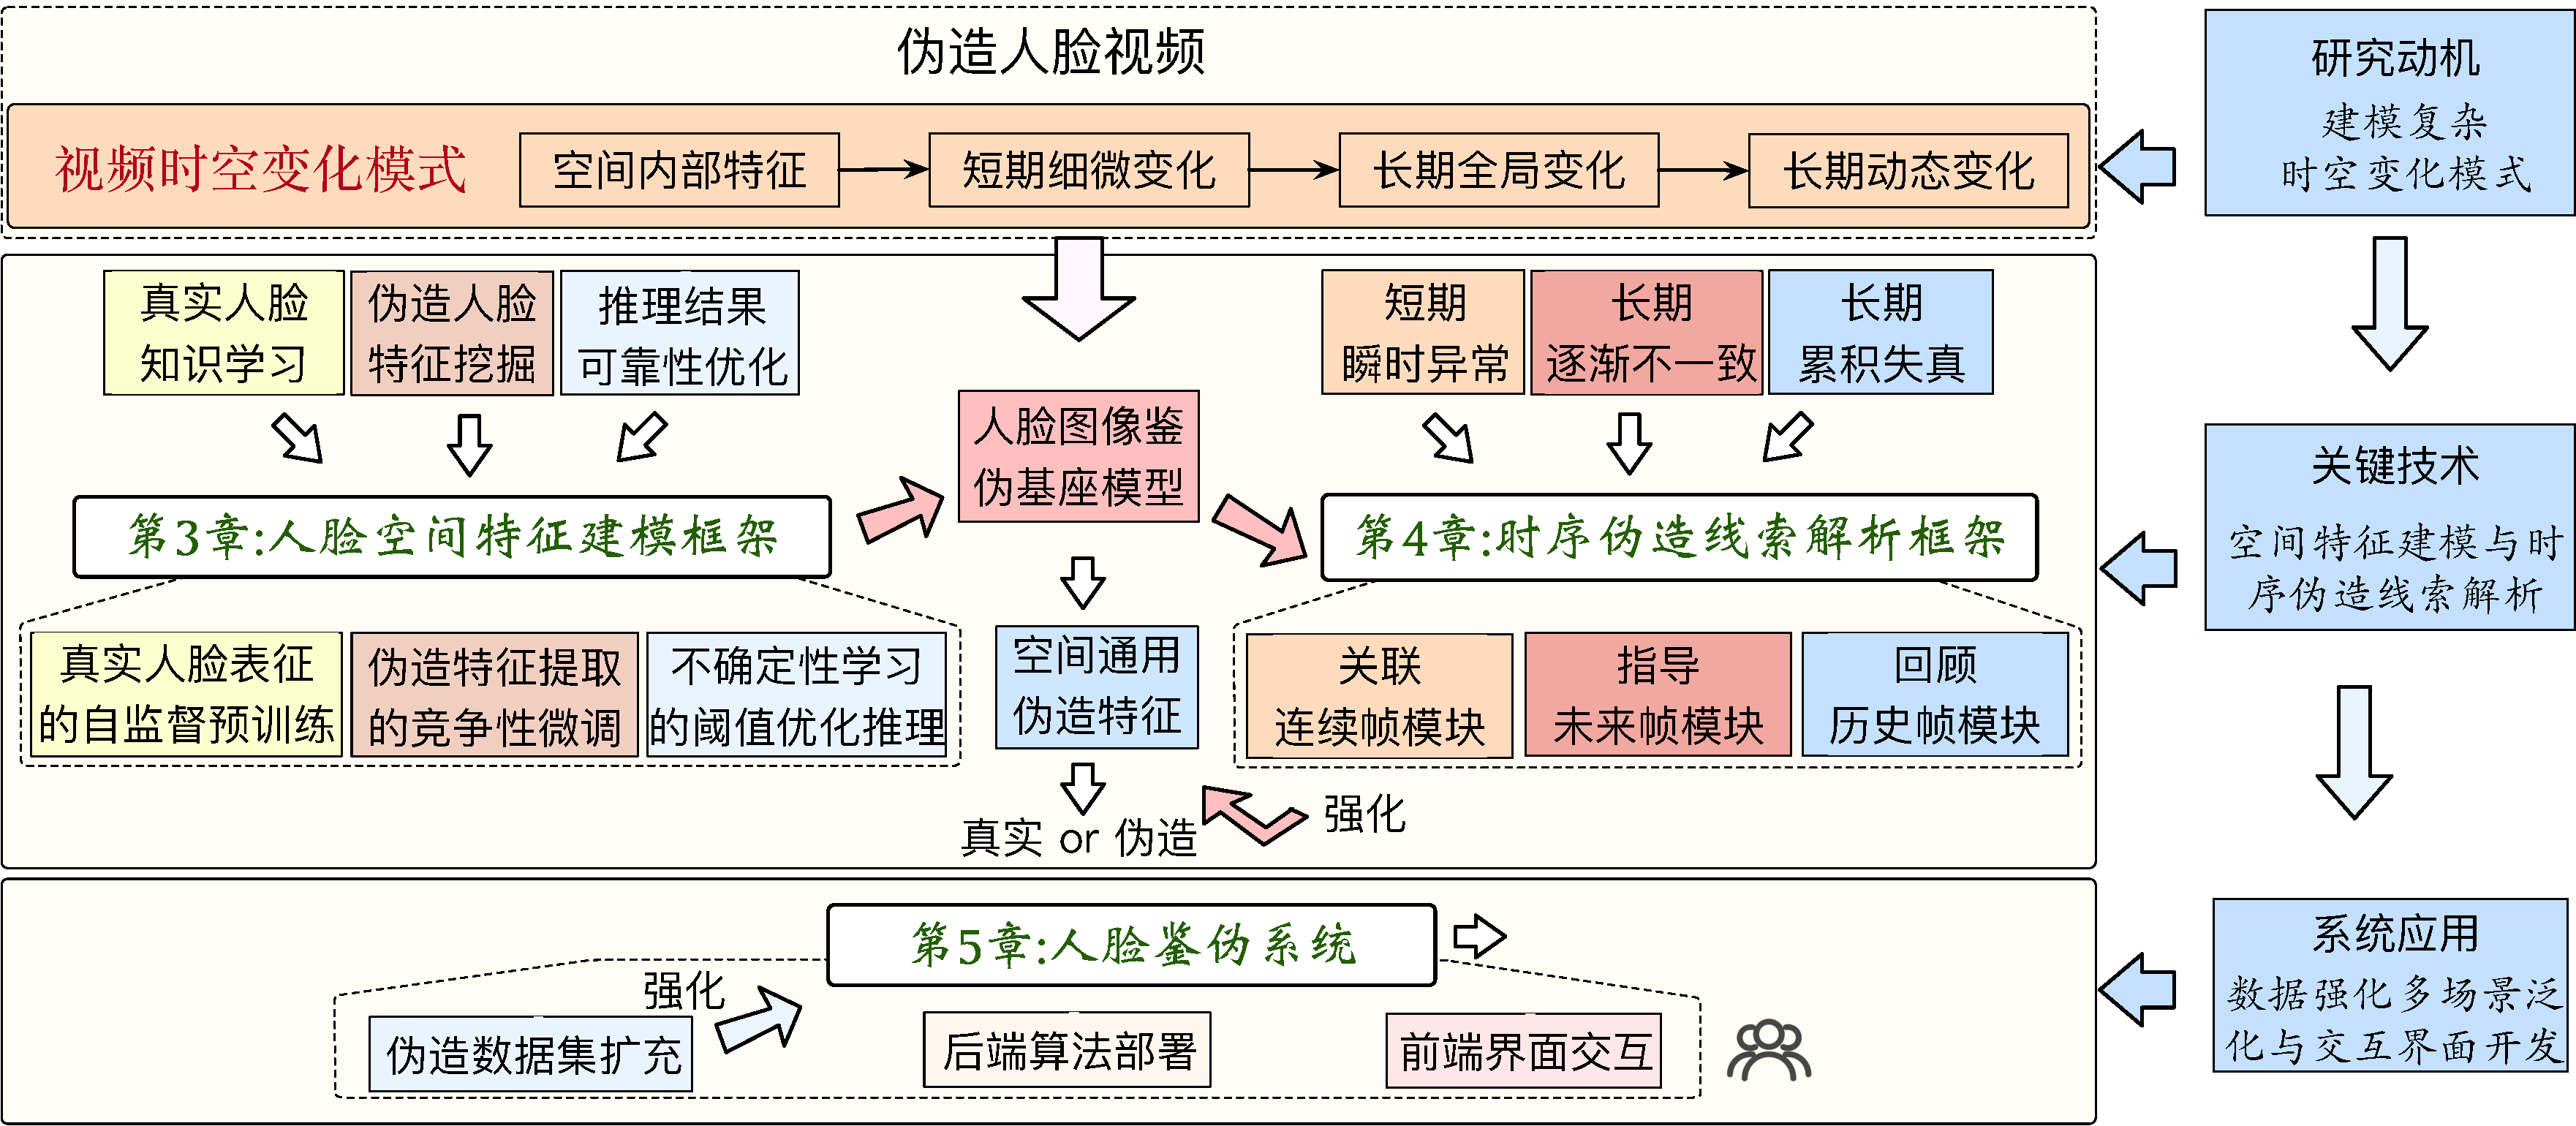
\includegraphics[width=1.0\linewidth]{fig/绪论.pdf}
\caption{本文的研究内容概览图}
\par\vspace{5pt}
\caption*{Figure \thefigure \ \ \ Overview of the research content of this thesis}
\label{fig:1-overview}
\end{figure}
\section{课题来源}
\esection{Research support}
国家自然科学基金面上项目“***”（批准号：***）。
\section{论文组织结构}
\esection{Paper structure}
本文聚焦于**，旨在**。组织结构如下：


第一章为绪论。首先介绍**任务的研究背景和意义；接着对国内外相关领域的研究现状和不足进行介绍；最后阐述本文的主要内容和贡献。



